%!TEX program = xelatex
\documentclass[a4paper,UTF8]{article}
\usepackage{ctex}
\usepackage[margin=1.25in]{geometry}
\usepackage{color}
\usepackage{graphicx}
\usepackage{amssymb}
\usepackage{amsmath}
\usepackage{amsthm}
\usepackage{enumerate}
\usepackage{bm}
\usepackage{hyperref}
\usepackage{epsfig}
\usepackage{color}
\usepackage{mdframed}
\usepackage{lipsum}
\usepackage{graphicx}
\usepackage{float}
\newmdtheoremenv{thm-box}{Theorem}
\newmdtheoremenv{prop-box}{Proposition}
\newmdtheoremenv{def-box}{定义}

\usepackage{listings}
\usepackage{xcolor}
\lstset{
	numbers=left,
	numberstyle= \tiny,
	keywordstyle= \color{ blue!70},
	commentstyle= \color{red!50!green!50!blue!50},
	frame=shadowbox, % 阴影效果
	rulesepcolor= \color{ red!20!green!20!blue!20} ,
	escapeinside=``, % 英文分号中可写入中文
	xleftmargin=2em,xrightmargin=2em, aboveskip=1em,
	framexleftmargin=2em
}

\usepackage{booktabs}

\setlength{\evensidemargin}{.25in}
\setlength{\textwidth}{6in}
\setlength{\topmargin}{-0.5in}
\setlength{\topmargin}{-0.5in}
% \setlength{\textheight}{9.5in}
%%%%%%%%%%%%%%%%%%此处用于设置页眉页脚%%%%%%%%%%%%%%%%%%
\usepackage{fancyhdr}
\usepackage{lastpage}
\usepackage{layout}
\footskip = 12pt
\pagestyle{fancy}                    % 设置页眉
\lhead{2021年春季}
\chead{模式识别}
% \rhead{第\thepage/\pageref{LastPage}页}
\rhead{作业三}
\cfoot{\thepage}
\renewcommand{\headrulewidth}{1pt}  			%页眉线宽,设为0可以去页眉线
\setlength{\skip\footins}{0.5cm}    			%脚注与正文的距离
\renewcommand{\footrulewidth}{0pt}  			%页脚线宽,设为0可以去页脚线

\makeatletter 									%设置双线页眉
\def\headrule{{\if@fancyplain\let\headrulewidth\plainheadrulewidth\fi%
\hrule\@height 1.0pt \@width\headwidth\vskip1pt	%上面线为1pt粗
\hrule\@height 0.5pt\@width\headwidth  			%下面0.5pt粗
\vskip-2\headrulewidth\vskip-1pt}      			%两条线的距离1pt
 \vspace{6mm}}     								%双线与下面正文之间的垂直间距
\makeatother

%%%%%%%%%%%%%%%%%%%%%%%%%%%%%%%%%%%%%%%%%%%%%%
\numberwithin{equation}{section}
%\usepackage[thmmarks, amsmath, thref]{ntheorem}
\newtheorem{theorem}{Theorem}
\newtheorem*{definition}{Definition}
\newtheorem*{solution}{Solution}
\newtheorem*{prove}{Proof}
\newcommand{\indep}{\rotatebox[origin=c]{90}{$\models$}}

\usepackage{multirow}

%--

%--
\begin{document}
\title{模式识别\\
作业三}
\author{181220076, 周韧哲, 本科,人工智能学院,人工智能学院选课}
\maketitle

\section*{Problem 1}
\begin{enumerate}[(a)]
	\item 设$A$的列秩为$r$,则$A$的列空间的维度是$r$,令$c_1,\cdots,c_r$为$A$的列空间的一组基,构成$m\times r$的矩阵$C$的列向量$C=[c_1,\cdots,c_r]$,并使得$A$的每个列向量是$C$的$r$个列向量的线性组合,由矩阵乘法定义,存在一个$r\times n$的矩阵$R$使得$A=CR$。可见$A$ 的每个行向量是$R$的行向量的线性组合,从而$A$的行秩小于等于$R$的行秩,而$R$的行秩小于等于其行数$r$(等于$A$的列秩),所以$A$的行秩小于等于$A$的列秩。同理可证$A$的列秩小于等于$A$的行秩,所以$A$的行秩等于列秩,因此$rank(X)=rank(X^T)$。
	\item 由于$A$的行秩小于等于行数$m$,$A$的列秩小于等于列数$n$,而行秩等于列秩,所以$rank(A)\leq m, rank(A)\leq n$,所以$rank(A)\leq \min(m,n)$。
	\item 设$X,Y$的秩分别为$s,r$,其列向量的极大线性无关向量组分别为$x_1,\cdots,x_s$和$y_1,\cdots,y_r$,则$X+Y$中任意列向量可以由$<x_1,\cdots,x_s,y_1,\cdots,y_r>$表示出,从而$rank(X+Y)\leq rank(X)+rank(Y)$。
	\item 令$U=XY$,则U的每个行向量是Y的行向量的线性组合,从而U的行秩小于等于Y的行秩;U的每个列向量是X的列向量的线性组合,从而U的列秩小于等于X的列秩,所以$rank(XY)\leq rank(X),rank(XY)\leq rank(Y)$,从而$rank(XY)\leq\min(rank(X), rank(Y))$。
	\item 令$N(\cdot)$表示零空间,则假设$a\in N(X)$,则有$Xa=0$,从而$X^TXa=0$,所以$N(X)\subseteq N(X^TX)$。假设$a\in N(X^TX)$,则有$X^TXa=0$,从而$a^TX^TXa=0$,即$(Xa)^T(Xa)=\|Xa\|_2^2=0$,所以$Xa=0$,所以$N(X^TX)\subseteq N(X)$。从而$N(X)=N(X^TX),dim(N(X))=dim(N(X^TX))$。由于$X$和$X^TX$都有$n$列,所以$rank(X)+dim(N(X))=n, rank(X^TX)+dim(N(X^TX))=n$,故$rank(X)=rank(X^TX)$。同理可证$rank(X^T)=rank((X^T)^TX^T)=rank(XX^T)$,所以$rank(X)=rank(XX^T)=rank(X^TX)$。
	\item 因为$rank(xx^T)\leq \min(rank(x),rank(x^T))=1$,所以当$x$为$0$向量时,$xx^T$为$0$矩阵,其秩为$0$,当$x$非$0$向量时,$xx^T$非$0$矩阵,其秩为$1$。因为实对称矩阵$A$一定与对角矩阵正交相似,即存在正交方阵$Q$使得$Q^{-1}AQ=\Lambda$,$\Lambda$为对角阵,对角元素为$A$的特征值,所以$A$的秩等于$\Lambda$的秩等于其非$0$特征值个数。
\end{enumerate}
\section*{Problem 2}
\begin{enumerate}[(a)]
    \item 由矩阵乘法公式,可以得出等式右边的乘法结果等于左边。
    \item 结果为$[v_1,\cdots, v_k,0,\cdots,0]_{n\times 1}$。
    \item 循环中的第$k$次会使得$A$的第$k$列的$k+1$位后的元素变为$0$,所以该算法会使得$A$成为上三角阵。
    \item 因为$M_k$为下三角矩阵,所以其行列式等于对角元素乘积,为$1$。从而$det(M_{n-1}M_{n-2}\cdots M_1)=det(M_{n-1})det(M_{n-2})\cdots det(M_1)=1$,且下三角矩阵的乘积仍然为下三角矩阵,即$L$为下三角矩阵。
    \item 由上面算法可知$A^{(n)}$为上三角阵,且$A^{(n)}=LA$,$A=L^{-1}A^{(n)}$,由$(d)$可知$L$为下三角矩阵且对角线元素为$1$,则$L^{-1}$为下三角矩阵且对角线元素为$1$,则满足$LU$分解,所以存在这样一个$LU$分解。假设分解结果不唯一,$A=L_1U_1=L_2U_2$,且$L_1,L_2,U_1,U_2$均可逆($A$非奇异),从而得到$L_1^{-1}L_2=U_1U_2^{-1}$,等式两边分别为下三角矩阵与上三角矩阵,且$L_1,L_2$对角线元素为$1$,所以$L_1^{-1}L_2=U_1U_2^{-1}=I$,即$L_1=L_2,U_1=U_2$。所以分解唯一。
    \item 由上题可知$A$存在唯一$LU$分解$A=LU$,且由于$A$为实对称正定矩阵所以$U$的对角线元素非$0$,则可将$U$分解为$U=DB$,其中$D=diag(u_{11},\cdots,u_{nn})$,$B$为上三角矩阵,对角元素为$1$,上三角中第$i$行从$1$开始后的元素为$[\frac{u_{i,i+1}}{u_{ii}},\frac{u_{i,i+2}}{u_{ii}},\cdots, \frac{u_{i,n}}{u_{ii}}]$。由于$A^T=A$,所以$(LDB)^T=B^TDL^T=LDB$,从而$L=B^T$,所以$A=LDL^T$,由$LU$分解唯一可得到$LDL$分解唯一性。
    \item 由上题知$A$存在唯一$LDL$分解,由于$A$正定,所以各阶顺序主子式均大于$0$,所以$D$对角元素为正数。所以可令$D=D^{\frac{1}{2}}D^{\frac{1}{2}}$,此时$A=LD^{\frac{1}{2}}D^{\frac{1}{2}}^TL^T=(LD^{\frac{1}{2}})(LD^{\frac{1}{2}})^T$,容易得知$LD^{\frac{1}{2}}$为下三角矩阵且对角元素为正,所以存在Cholesky分解$G=LD^{\frac{1}{2}}$,由$LDL$分解唯一性可得到Cholesky分解唯一性。
\end{enumerate}

\section*{Problem 3}
\begin{enumerate}[(a)]
    \item 已下载并编译,如下图所示。
    \begin{figure}[H]
		\centering
		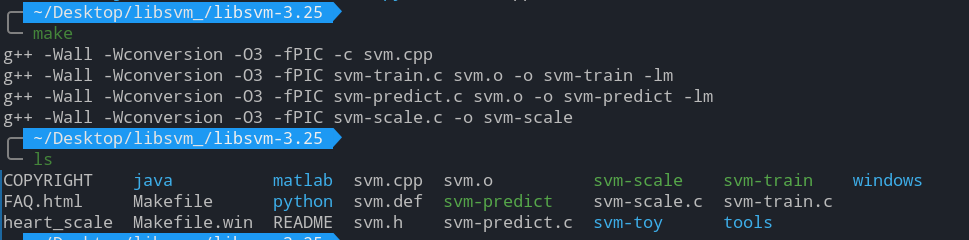
\includegraphics[width=0.5\textwidth]{pic/q1.png}
		\label{Fig.1}
	\end{figure}
    \item \begin{enumerate}[i.]
        \item 如下图,默认参数的准确率是$66.925\%$。
        \begin{figure}[H]
		\centering
		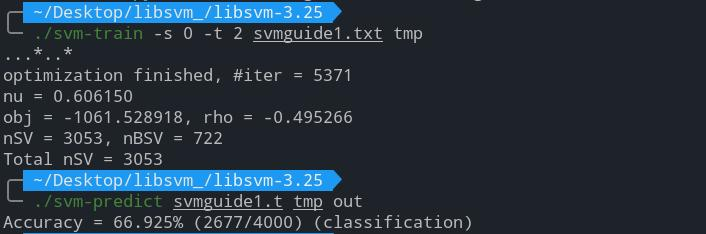
\includegraphics[width=0.5\textwidth]{pic/q2.png}
		\label{Fig.2}
	\end{figure}
        \item 如下图,准确率是$96.15\%$。
        \begin{figure}[H]
		\centering
		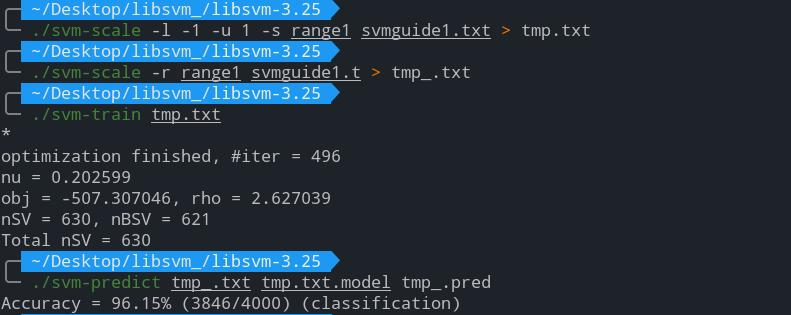
\includegraphics[width=0.5\textwidth]{pic/q3.png}
		\label{Fig.2}
	\end{figure}
        \item 如下图,准确率是$95.675\%$。
        \begin{figure}[H]
		\centering
		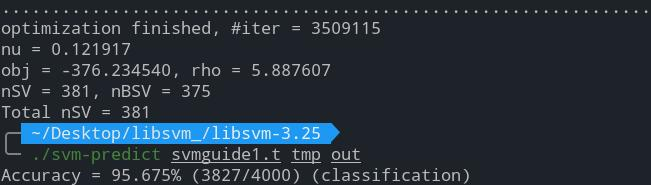
\includegraphics[width=0.5\textwidth]{pic/q4.png}
		\label{Fig.2}
	\end{figure}
        \item 如下图,准确率是$70.475\%$。
        \begin{figure}[H]
		\centering
		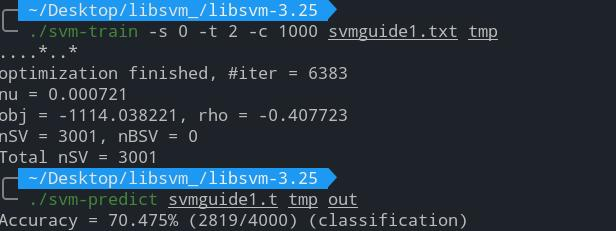
\includegraphics[width=0.5\textwidth]{pic/q5.png}
		\label{Fig.2}
	\end{figure}
        \item 使用easy.py工具确认得到$C=2, \gamma=2$,训练得到准确率是$96.875\%$。
    \end{enumerate}
    我认识到不同超参、核函数以及数据是否规范化对模型的效果有很大的影响,需要仔细确认合适的超参数和合适的方法才能较好地提高模型准确率。
    \item 找到不平衡数据集svmguide3,在默认参数下准确率很低仅有$2\%$,使用$-wi$参数将第一类赋予权重,随着权重增大模型准确率也在提高,当权重赋予到$6$时准确率达到$100\%$,所以$-wi$参数在不平衡数据集上非常有用。实验结果如下图。
    \begin{figure}[H]
		\centering
		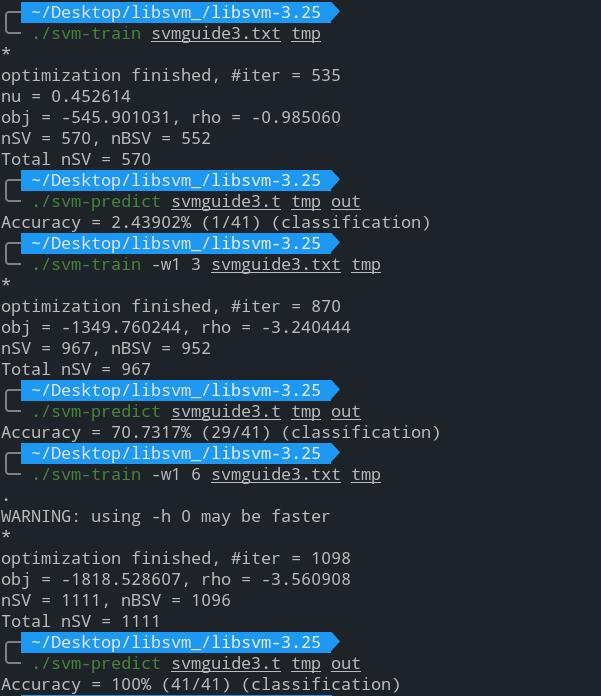
\includegraphics[width=0.5\textwidth]{pic/q7.png}
		\label{Fig.2}
	\end{figure}
\end{enumerate}

\section*{Problem 4}
\begin{enumerate}[(a)]
    \item 因为$\kappa_{HI}(x,y)=\sum_{i=1}^d\min(x_i,y_i)=\sum_{i=1}^d\min(y_i,x_i)=\kappa_{HI}(y,x)$,所以该核函数对称。对于样本集$D=x_1,\cdots,x_n$,设$\kappa_{HI}(\cdots,\cdots)$对应的核矩阵为$K$。对于任意向量$z\in\mathbb{R}^n$
    \begin{align*}
        z^TKz &= \sum_{p=1}^n\sum_{q=1}^n z_pK_{ij}z_q\\
        &= \sum_{p=1}^n\sum_{q=1}^n z_pz_q\sum_{i=1}^d\kappa_{HI}(x_{pi},x_{qi})\\
        &= \sum_{i=1}^d\sum_{p=1}^n\sum_{q=1}^n z_pz_q\kappa_{HI}(x_{pi},x_{qi})\\
        &=\sum_{i=1}^dz^TK_{i}'z
    \end{align*}
    其中$K'_{i}$为样本集$D$中向量的第$i$个元素作为样本集生成的核矩阵,由于$\kappa_{HI}$对于任意标量都是合法的核函数,所以其对应核矩阵$K'$半正定,所以$z^TK'_{i}z\geq0,i=1,\cdots,n$,所以$z^TKz\geq 0$,所以$\kappa_{HI}$对非负向量$x,y$也是一个合法核函数。
    \item 易得矩阵$Y$可由$X$同过一系列对应的行变换和列变换得到,即$Y=P^TXP$,$P$为若干个初等矩阵的乘积,且$P$可逆。当$X$正定时,对任意向量$z$有$z^TYz=(Pz)^TX(Pz)>0$,所以$Y$也正定;当$Y$正定时,对任意向量$z$有$z^TXz=(P^{-1}z)^TX(P^{-1}z)>0$,所以$X$也正定。同理可得$X$半正定当且仅当$Y$半正定。
    \item 我们可将矩阵$X$初等变换来对角化,每一行减去上一行,每一列减去上一列来使得其成为对角矩阵$A$,由于该矩阵为排列形成的,所以有$x_{ij}<=x_{pq},p>=i,q>=j$,从而$A$的对角元素非负,且可表示成一系列初等矩阵的乘积:$A=P^TXP$,其形如LDL分解,$L=P^T$。因为$A$的对角元素非负所以其半正定,由上题结论知$A$半正定当且仅当$X$半正定,所以$X$半正定。
    \item 易知只需证明对两正标量$x,y$有$\min(x,y)\leq\frac{2xy}{x+y}$,则$\kappa_{HI}\leq\kappa_{\mathcal{X}^2}$成立。当$\min(x,y)=x$时,易得$\min(x,y)=x=\frac{x(x+y)}{x+y}\leq\frac{x(y+y)}{x+y}=\frac{2xy}{x+y}$,当$\min(x,y)=y$时同理,所以$\kappa_{HI}\leq\kappa_{\mathcal{X}^2}$。
    \item 因为$\kappa_{HE}(x,y)=\sum_{i=1}^d\sqrt{x_iy_i}=\sum_{i=1}^d\sqrt{y_ix_i}=\kappa_{HE}(y,x)$,所以该核函数对称。可构造映射$\phi(x)=(\sqrt{x_1},\cdots,\sqrt{x_n})$,满足$\kappa_{HE}(x,y)=\phi(x)^T\phi(y)$,所以$\kappa_{HE}$为合法核函数。为了证明$\kappa_{HE}\geq\kappa_{\mathcal{X}^2}$,易知只需证明对两正标量$x,y$有$\sqrt{(x,y)}\geq\frac{2xy}{x+y}$,则$\kappa_{HE}\geq\kappa_{\mathcal{X}^2}$成立。由基础不等式得$\frac{1}{x}+\frac{1}{y}\geq2\sqrt{\frac{1}{xy}}$,从而$\sqrt{(x,y)}\geq\frac{2}{\frac{1}{x}+\frac{1}{y}}=\frac{2xy}{x+y}$,所以$\kappa_{HE}\geq\kappa_{\mathcal{X}^2}$。
    \item 不妨设$\|x\|_\infty=\max_{1\leq i\leq d}|x_i| \leq a$,即$x$每一维度的最大值不超过$a$,则取映射$\phi:\mathbb{N}^d\rightarrow \{0,1\}^{ad}$,$\phi_i(x_i)=(1,\cdots,1,0,\cdots,0)$,即将$x_i$表示为长度为$a$的二值向量,其中$1$的个数恰好等于$x_i$的数值,容易看出对于标量$x,y$,$\phi_i(x)^T\phi_i(y)=\min(x,y)$,则可构造$\phi(x)=(\phi_1(x_1)\cdots \phi_d(x_d))$,所以$\phi(x)^T\phi(y)=\sum_{i=1}^d\min(x_i,y_i)=\kappa_{HI}(x,y)$。
\end{enumerate}

\section*{Problem 5}
\begin{enumerate}[(a)]
    \item LLE的目标为$\min E=\sum_{i=1}^n e_i=\sum_{i=1}^n W_i^T(x_i-x_j)(x_i-x_j)^TW_i$,其中$W_i=(w_{i1},\cdots,w_{ik})^T$为$k$个近邻样本权重,$Z_i=(x_i-x_j)(x_i-x_j)^T$,$x_j$属于$x_i$的$k$个近邻,则约束等于$\sum_{j=1}^nw_{ij}=W_i^Te=1$,$e$为$k$维全$1$向量。根据拉格朗日乘子法可得目标函数$L(W)=\sum_{i=1}^kW_i^TZ_iW_i+\lambda (W_i^Te-1)$
    ,求导可得$W_i=\frac{Z_i^{-1}e}{e^TZ_i^{-1}e}$。
    \item \begin{enumerate}[i.]
             \item 因为\begin{align*}
                 e_i&=\|Q(x_i-\sum_{j=1}^nw_{ij}x_j)\|^2\\
                 &=(x_i-\sum_{j=1}^nw_{ij}x_j)^TQ^TQ(x_i-\sum_{j=1}^nw_{ij}x_j)\\
                 &=(x_i-\sum_{j=1}^nw_{ij}x_j)^T(x_i-\sum_{j=1}^nw_{ij}x_j)\\&=e_i
             \end{align*}
             所以旋转不变。
             \item 因为\begin{align*}
                 e_i&=\|(x_i+t)-\sum_{j=1}^nw_{ij}(x_j+t)\|^2\\
                 &=\|x_i-\sum_{j=1}^nw_{ij}x_j+t-\sum_{j=1}^nw_{ij}t\|^2\\
                 &=e_i
             \end{align*}
             所以平移不变。
             \item 因为\begin{align*}
                 e_i&=\|sx_i-\sum_{j=1}^nw_{ij}sx_j\|^2\\
                 &=\|s(x_i-\sum_{j=1}^nw_{ij}x_j)\|^2\\
                 &=s^2e_i
             \end{align*}
             相当于给目标函数乘了个正系数,不影响优化结果,所以缩放不变。
          \end{enumerate}
    \item $w_{ij}$是重构$x_i$中的向量$x_j$的线性权重,反应了$x_i$与其近邻样本的关系,所以通过这近邻权重去求解$x_i$的重构表示$y_i$能够保持样本局部关系,从而保持局部几何性质。$\sum_{i=1}^ny_i=0$消去了平移自由度,$\sum_{i=1}^ny_iy_i^T=I$消去了缩放自由度,由$(b)$可知旋转自由度仍存在且不会对新的表示产生负面影响。
    \item 令$\mathcal{L}=\sum_{i=1}^n\|\mathbf{y}_i-\sum_{j=1}^nw_{ij}\mathbf{y}_j\|^2=\sum_{i=1}^n\|(1-w_{ii})\mathbf{y}_i+\sum_{j=1,j\neq i}^n(-w_{ij})\mathbf{y}_j\|^2$,容易看出$(1-w_{ii})\mathbf{y}_i+\sum_{j=1,j\neq i}^n(-w_{ij})\mathbf{y}_j=\sum_{j=1}^{n}(I-W)_{ij}\mathbf{y}_j$,所以
    \begin{align*}
        \mathcal{L}&=\sum_{i=1}^n\|\sum_{j=1}^{n}(I-W)_{ij}\mathbf{y}_j\|^2\\
        &=\sum_{i=1}^n\sum_{j=1}^{n}\sum_{k=1}^n(I-W)_{ij}(I-W)_{ik}\mathbf{y}_j^T\mathbf{y}_k\\
        &=\sum_{j=1}^{n}\sum_{k=1}^n(\sum_{i=1}^n(I-W)_{ij}(I-W)_{ik}\mathbf{y}_j^T\mathbf{y}_k)\\
        &=\sum_{j=1}^{n}\sum_{k=1}^nM_{jk}\mathbf{y}_j^T\mathbf{y}_k\\
        &=\sum_{i=1}^{n}\sum_{j=1}^nM_{ij}\mathbf{y}_i^T\mathbf{y}_j
    \end{align*}
    \item \begin{enumerate}[1)]
        \item 对任意向量$x$,$x^TMx=x^T(I-W)^T(I-W)x=\|(I-W)x\|^2\geq0$,所以$M$半正定。
        \item $M_{ij}=\sum_{k=1}^{n}(I-W)_{ik}^T(I-W)_{kj}=\sum_{k=1}^n(w_{ik}w_{kj})-2w_{ij}$,$M\mathbf{1}=\mathbf{0}=M_{:1}+\cdots+M_{:n}$的第$i$个元素为$\sum_{j=1}^nM_{ij}=\sum_{j=1}^n\sum_{k=1}^nw_{ik}w_{kj}-2\sum_{j=1}^nw_{ij}+1=\sum_{j=1}^nw_{kj}\sum_{k=1}^nw_{ik}-1=0$,
        则有$M\mathbf{1}=\mathbf{0}$,即$\mathbf{1}$为特征值为$0$的特征向量。
    \end{enumerate}
    证明$E_d$满足两个约束条件:
    \begin{enumerate}[1)]
        \item 已知$\mathbf{1}$为特征向量,由特征向量正交可得$\sum_{k=1}^n\xi_i^{k}=0,i=2,\cdots,d+1$,即$E_d$的行向量之和等于$\mathbf{0}$,满足第一个约束。
        \item $\sum_{i=1}^ny_iy_i^T$的对角元素为$\sum_{i=1}^n(y_i^{j})^2=\sum_{i=1}^n(\xi_j^{i})^2=1,j=1,\cdots,d$,所以对角元素为$1$。非对角线元素有$\sum_{i=1}^ny_i^{j}y_i^k=\sum_{i=1}^n\xi_j^{i}\xi_k^i=0$。所以$\sum_{i=1}^ny_iy_i^T=I$,满足第二个约束条件。舍弃$\xi_1$可使得$y_i$均值为$0$,满足第一个约束。
    \end{enumerate}
    \item 已浏览。
\end{enumerate}
\end{document}